\section{Methods}\label{methods}

\subsection{Study area and sampling design}

We conducted five sampling campaigns across the Rub' al-Khali along
a transect from the western escarpment (19.15\degree N, 45.17\degree
E) to the eastern border of Saudi Arabia with Oman (20.71\degree N,
54.73\degree E). The 60 ordered sampling sites yield a 1,043-km
cumulative path and lie 1,015~km apart end to end.
Figure~\ref{fig:transect} shows the site coordinates and altitude
profile. Cumulative distance sums great-circle distances between
successive sites, using an Earth radius of 6,371~km.

\begin{figure}[!htbp]
  \centering
  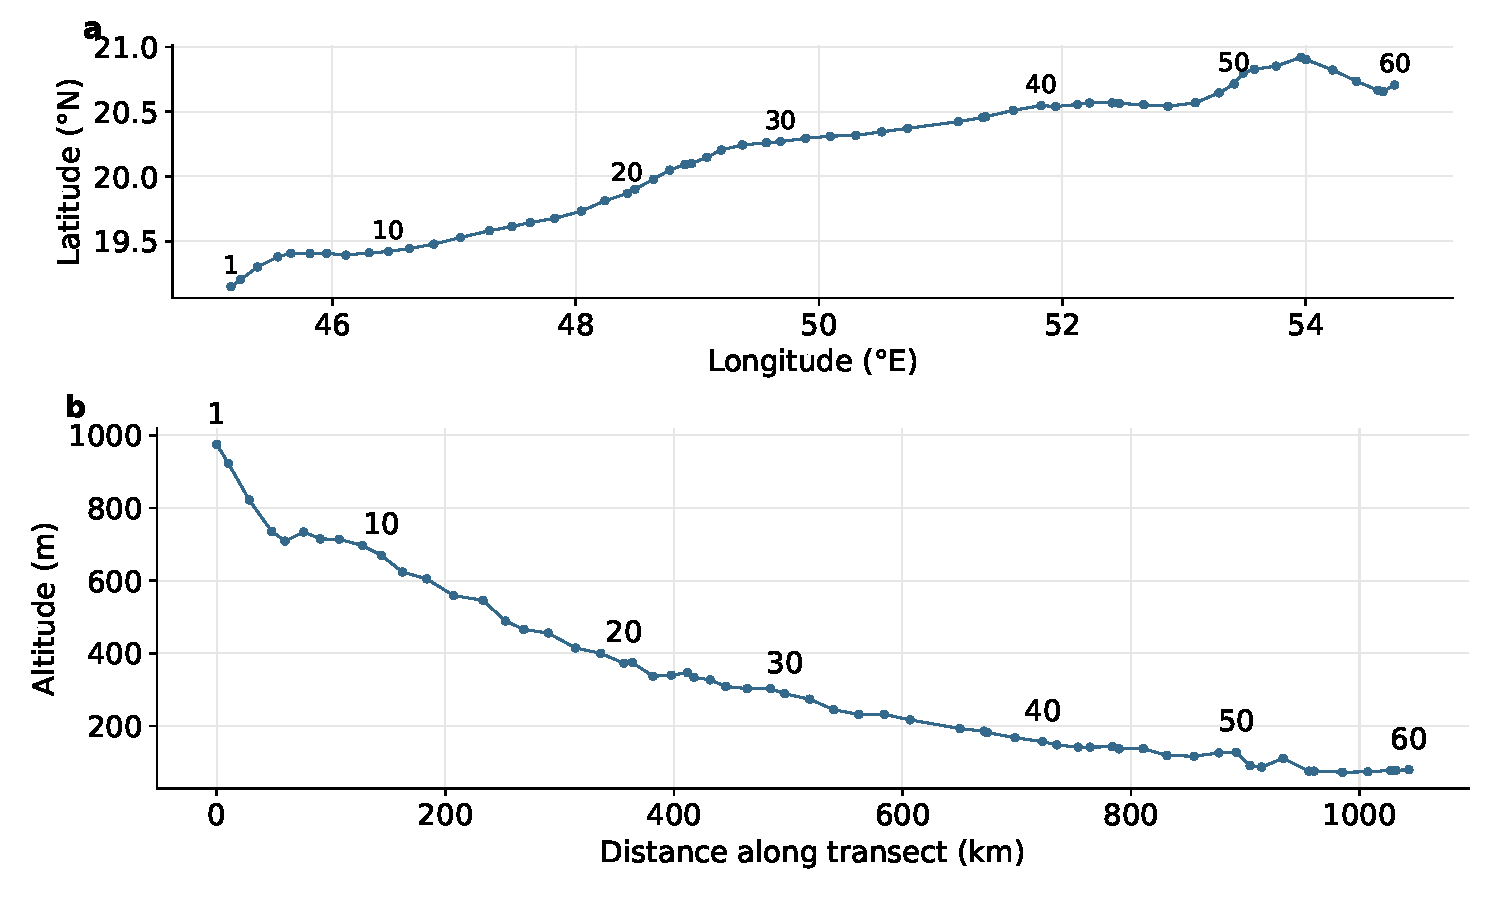
\includegraphics[width=\textwidth]{figures/transect/transect_altitude.pdf}
  \caption{Primary sampling transect across the Rub' al-Khali.
    Panel a shows the coordinates of sites 1--60; panel b shows their
    archived altitude values against cumulative great-circle distance
    in site order. Labels identify selected sites. Coordinates and
    altitude come from the versioned site-altitude table; the
    historical elevation source and vertical datum remain undocumented.}
  \label{fig:transect}
\end{figure}

The transect comprises 60 primary sampling sites at predetermined
coordinates and 10 named locations, including wells, a hot spring and
an oil-spill site. Trip~1 source identifiers 61--64 are aliases for four
named catalogue locations, established by coordinate matching.
The repeated-campaign analytical frame uses sites~1--60.
We preserve source sheets and apply the versioned correction ledger
to generate curated metadata.

To capture temporal variability, we conducted campaigns across
different seasons: late winter 2023 (Trip 1, 64 sites visited), summer
2023 (Trip 2, truncated to 8 sites due to extreme temperatures),
winter 2024 (Trip 3, 65 sites visited), summer 2024 (Trip 4, 60 sites
visited), and autumn 2025 (Trip 5, 62 sites visited). Field sheets provide temperature, atmospheric pressure and relative
humidity with campaign-specific availability. We summarize the
observational coverage in Table~\ref{tab:env_summary}. %, although the available measurements differ by campaign.
We acquired handheld field XRF measurements during Trip~5 and
laboratory XRF measurements of archived material from all five
campaigns. The curated environmental table retains 274 nonblank
source rows. Of these, 260 resolve to catalogue site visits and
generate 260 temperature, 187 pressure and 251 humidity values.
Fourteen auxiliary or revisit labels remain table-only pending
unambiguous site identification. The correction ledger assigns the
eight Trip~2 values 34.5--41.9 to temperature using their worksheet
context and the field note; pressure and humidity remain missing.
The Trip~5 site~40 humidity value of 194\% is retained in the source
ledger and excluded from the curated measurements.

\begin{table}[h]
  \centering
  \caption{Coverage of field environmental logs. Numeric identifiers, named
    locations and auxiliary observations retain separate source labels.}
  \label{tab:env_summary}
  \small
  \setlength{\tabcolsep}{3pt}
  \begin{tabular}{lllc}
    \toprule
    Campaign & Season & Field-log records & Measurements available \\
    \midrule
    Trip 1 & Late Winter 2023 & 1--60; 4 named; 15 auxiliary$^\ast$ & Temp, Press, Hum. \\
    Trip 2 & Summer 2023 & 1--8 & Temp. \\
    Trip 3 & Winter 2024 & 1--60; 5 named & Temp, Press, Hum. \\
    Trip 4 & Summer 2024 & 1--60 & Temp, Hum. \\
    Trip 5 & Autumn 2025 & 1--60; 2 named & Temp, Press, Hum. \\
    \bottomrule
  \end{tabular}
  \parbox{0.94\columnwidth}{\footnotesize $^\ast$The 15 records are appended
    to the legacy Trip~3 worksheet but are dated March 2023 in the
    original workbook and are curated as Trip~1 auxiliary/revisit
    observations.}
\end{table}



The sampling design targeted three soil
compartments: bulk surface soil, bulk subsurface soil
(5--10 cm depth, hereafter ``deep''), and subsurface soil collected
near roots (5--10 cm depth, hereafter ``root-adjacent''). 
The legacy class label Deep Soil Sample denotes the 5--10~cm
bulk compartment, called shallow-subsurface in the companion
ecology analysis \cite{ecology_companion}. We collected three
co-located field replicates per compartment using sterile tubes and
sterile plastic spoons. From Trip~2 onwards, three adjacent tubes
were taped or chained together for collection, so adjacent sampling
positions were separated by one external tube diameter. Trip~5
used larger tubes. Exact tube diameters, surface sampling depth
and distance from roots were unrecorded. These co-located
replicates share a site and compartment.
We preserved samples at $-20$\degree C in the field
using an Engel MR040F portable freezer. At the end of each campaign,
we transferred samples to an $-80$\degree C freezer in the laboratory.

The source ledger additionally contains 248 plant entries linked by
campaign, site and source identifier. Tissue type, host-identification
procedure, vouchers and plant-specific storage details are incomplete
in the archived protocol. These entries preserve plant provenance;
root-adjacent soil retains its own specimen identity.

\begin{table}[h]
\centering
\caption{Source-specimen coverage by campaign and soil compartment,
generated from \texttt{evidence/release/sample\_ledger.tsv}.
All catalogue sites are included; plant and control rows are excluded.
Columns count source rows eligible for specimen representation,
expected by the extract generator, linked to at least one run,
present in the ASV table and retained in the ecological analysis.
Repeated sequencing profiles can share one source-specimen row.}
\label{tab:sample_coverage}
\small
\setlength{\tabcolsep}{3pt}
% Generated by scripts/manuscript/generate_sample_coverage.py
\begin{tabular}{llrrrrr}
\toprule
Trip & Compartment & Specimens & Extract-linked & Run-linked & ASV table & Ecology \\
\midrule
1 & Subsurface & 192 & 184 & 111 & 110 & 108 \\
1 & Root-adjacent & 192 & 170 & 102 & 106 & 104 \\
1 & Surface & 192 & 185 & 108 & 114 & 113 \\
2 & Subsurface & 24 & 23 & 9 & 8 & 7 \\
2 & Root-adjacent & 24 & 18 & 13 & 13 & 11 \\
2 & Surface & 24 & 22 & 7 & 6 & 6 \\
3 & Subsurface & 180 & 180 & 141 & 141 & 141 \\
3 & Root-adjacent & 180 & 174 & 154 & 154 & 154 \\
3 & Surface & 180 & 180 & 156 & 155 & 155 \\
4 & Subsurface & 180 & 63 & 59 & 59 & 59 \\
4 & Root-adjacent & 180 & 60 & 58 & 58 & 58 \\
4 & Surface & 180 & 62 & 60 & 60 & 60 \\
5 & Subsurface & 180 & 93 & 57 & 55 & 55 \\
5 & Root-adjacent & 180 & 151 & 133 & 133 & 133 \\
5 & Surface & 180 & 82 & 30 & 29 & 29 \\
\bottomrule
\end{tabular}

\end{table}

\subsection{Laboratory controls}

Control coverage differed by campaign and processing stage
(Table~\ref{tab:controls}). Extraction blanks underwent the same
procedure as biological specimens. Trips~4--5 used one blank per
trip-specific extraction-day batch. Trips~1--3 used one blank per
extraction kit, and Trips~1--2 included shared extraction days.
The PowerSoil Pro control has a sequencing record
(\texttt{Extraction-Ctrl-Pro-Trip1}, library \texttt{M-25-0929});
the PowerSoil blank is present in laboratory records, with no matching
sequencing record located in the available sheets.

\begin{table}[h]
\centering
\caption{Control coverage relevant to the released amplicon data.
Detailed material and sequence occurrences are retained in the control
registry.}
\label{tab:controls}
\small
\setlength{\tabcolsep}{3pt}
\begin{tabular}{p{0.12\textwidth}p{0.25\textwidth}p{0.25\textwidth}p{0.26\textwidth}}
\toprule
Campaign & Extraction controls & PCR-stage negatives & Sequenced standards \\
\midrule
1 & Per-kit; Pro blank sequenced & Nuclease-free water & Identity unresolved \\
2 & Shared per-kit coverage & NTC-2 & Two purified-DNA standards \\
3 & Per-kit coverage & PCRCtrl, index 728 & Two whole-cell standards \\
4 & Six sequenced blanks; three unsequenced batches & PCR blank and NTC unsequenced & Amplification-positive control only \\
5 & 18 canonical blank profiles; 17 batch-linked & Six canonical NTC profiles & Field standard sequenced by shotgun \\
\bottomrule
\end{tabular}
\end{table}

The canonical table contains 18 Trip~5 extraction-blank profiles
(EB1--EB18) and six no-template PCR controls
(Negative1, Negative2, Negative4--Negative7). Seventeen extraction
blanks have confirmed batch links to 217 biological profiles.
The six Trip~4 extraction blanks (SEB, EB1--EB5) were sequenced on
a shared run and denoised separately with the same pipeline on
30~August 2026. Three of the nine Trip~4 extraction batches had
unsequenced blanks, leaving complete or partial coverage gaps at
28 sites. The corrected batch workbook supplies specimen-level
membership; the source-to-profile ledger also excludes unsequenced
S34Dr1 and S40PRr1. S40PRr1 failed three amplification attempts.
S34Dr1 yielded DNA but was probably missed during pooling.

No-template controls contained PCR reagents and molecular-grade water
in place of template DNA. Reagent-only PCR blanks contained neither
added water nor template. One reagent-only blank was prepared per
amplification plate. Most showed low or undetectable concentration
and adapter-dimer-dominated TapeStation profiles and were excluded
from sequencing. Trip~5 reagent-only blanks were lost during
handling, attributed to evaporation. Trip~4's PCR blank and NTC were
excluded because their index pairs conflicted with biological
libraries on the shared run. The Trips~1--3 control libraries were
sequenced on NovaSeq~6000 A01018 run~321, flowcell HVJY5DRX3, and
denoised with biological libraries in July 2025; they are distributed
separately from the canonical feature table. Re-denoising on
30~August 2026 supplied the control comparison in Technical Validation.

Positive standards were reserved for genus-recovery evaluation.
Trips~1--2 used the ZymoBIOMICS HMW DNA Standard D6322, introduced
at PCR; Trip~3 used the whole-cell D6300 Microbial Community Standard,
which also undergoes extraction. Trip~4 had a laboratory
amplification-positive control assessed by gel electrophoresis and
TapeStation, and Trip~5's field D6300 standard was sequenced by
shotgun metagenomics. Four sequenced standards from Trips~2--3
support the amplicon genus-recovery analysis. The Trip~1 FPosCtrl1
identity remains unresolved because its index and well disagree, so
it remains excluded.

D6322 contains seven bacterial genomes at 14\% genomic DNA each and
one yeast at 2\%; D6300 contains eight bacterial genomes at 12\% each
and two yeasts at 2\% each. These are manufacturer genomic-DNA mass
fractions. The recovery analysis compares expected and observed
bacterial genera, including unassigned reads and additional taxa.
Such departures can reflect processing contamination, amplification,
classification or index-assignment errors. The registry retains
intended materials, observed profiles and identity evidence separately.

\subsection{DNA extraction and sequencing}

Genomic DNA was extracted from 0.9--1.2~g of soil using either the
QIAGEN PowerLyzer PowerSoil Kit (catalogue no.\ 12855-50) or the QIAGEN
DNeasy PowerSoil Pro Kit (catalogue no.\ 47014). Both kits were used
in Trips~1--3: among the sequenced profiles, the sample ledger records
the PowerLyzer PowerSoil Kit for 77 Trip~1, 10 Trip~2 and 359 Trip~3
profiles (54 of the Trip~3 records name the MoBio PowerSoil kit) and
the DNeasy PowerSoil Pro Kit for 217 Trip~1, 11 Trip~2 and 87 Trip~3
profiles; 46 Trips~1--3 profiles have no recorded kit. The QIAcube
Connect was introduced for
routine extraction starting with Trip~4; samples from Trips~1--3 were
also processed using the QIAcube Connect when re-extraction was
required. The extraction method and re-extraction history were
recorded for each specimen when available.

Frozen soil samples were thawed on ice and processed immediately after
thawing. Before homogenization, samples were incubated at 65\degree C
for 10~min with agitation at 1,200~rpm, then homogenized using a
PowerLyzer 24 Homogenizer at 4,000~rpm for one 45-second cycle.
The remaining purification steps were performed either
manually or using a QIAcube Connect instrument, following the
manufacturer's protocol. DNA was eluted in 50~\textmu L of the elution
buffer supplied with the respective kit.

Extraction controls followed the campaign-specific scheme above.

Extracted DNA was quantified using the Qubit dsDNA High Sensitivity
assay, with fluorescence measured using a Varioskan LUX multimode
plate reader (Thermo Fisher Scientific). The project spreadsheet retains numerical extract concentrations. Progression to indexing and sequencing was
determined by an amplicon of the expected size after first-round PCR. DNA concentrations and processing information were recorded
in a central project spreadsheet. Extracted DNA was stored at
$-20$\degree C until PCR amplification.

The V3--V4 region of the bacterial 16S rRNA gene was amplified using
the Bakt\_341F (\texttt{CCTACGGGNGGCWGCAG}) and Bakt\_785R
(\texttt{GACTACHVGGGTATCTAATCC}) primers \cite{klindworth2013primers},
both carrying Illumina overhang adapters. First-round PCR was
performed using TaKaRa Ex Taq DNA Polymerase (catalogue no.\
RR001B). Each reaction had a total volume of 50~\textmu L and
contained 5~\textmu L of 10$\times$ buffer with Mg$^{2+}$,
4~\textmu L of dNTP mix (2.5~mM of each dNTP),
2~\textmu L of each 10~\textmu M primer stock, 0.25~\textmu L
of polymerase (5~U/\textmu L), 5~\textmu L of extracted DNA and 31.75~\textmu L
of nuclease-free water. The final primer concentration was
0.4~\textmu M per primer and 0.2~mM per dNTP, with 1.25~U
of polymerase per reaction. The PCR programme was: initial
denaturation at 95\degree C for 3~min; 35 cycles of 95\degree C for
10~s, 65\degree C for 30~s and 72\degree C for 1~min; and a final
extension at 75\degree C for 5~min.

First-round PCR products were assessed by electrophoresis on a 1\%
agarose gel. Samples showing an amplicon at the expected size of
approximately 500~bp were classified as passing and were then
indexed. Samples without a visible product were classified as failed;
these were re-amplified with 8~\textmu L and then 12~\textmu L of DNA,
with water reduced to 28.75~\textmu L and 24.75~\textmu L,
respectively. DNA input was set by volume because most extracts had low
or undetectable concentrations. Samples without a product after three
attempts were classified as failed; the earlier laboratory account also
documents re-extraction at the end of the workflow.

Dual indices and Illumina sequencing adapters were added in a
second-round PCR using the QIAGEN Multiplex PCR Kit (catalogue no.\
206143), following the Illumina 16S Metagenomic Sequencing Library
Preparation protocol \cite{illumina16S}: initial activation at
94\degree C for 15~min; 8 cycles of 94\degree C for 30~s, 55\degree C
for 30~s and 72\degree C for 30~s; final extension at 72\degree C for
5~min.

Indexed libraries were purified using Agencourt AMPure XP beads at a
0.8:1 bead-to-sample volume ratio,
quantified using the Qubit dsDNA High Sensitivity assay, and assessed
for fragment size using an Agilent 4200 TapeStation with the D5000
ScreenTape assay. Libraries were pooled by molarity calculated from
concentration and fragment size in the Core Lab pooling sheet.
Supplementary Section~S2 specifies the
pooling calculation and the remaining run-specific metadata gaps.
Amplicon pools were sequenced on an Illumina NovaSeq~6000 using
an SP flow cell with a 500-cycle reagent kit to generate
$2 \times 250$~bp
paired-end reads. Sample processing and library preparation were
performed in the PI's laboratory and sequencing was conducted at the
Bioscience Core Lab at KAUST.


\subsection{Sequencing data processing}

We processed raw amplicon reads with nf-core/ampliseq (v2.14.0)
\cite{nfcore, ampliseq}, applying the DADA2 algorithm \cite{dada2} for error
correction and denoising, and assigning taxonomy against the SILVA
database (v138.2) \cite{silva}. The submission records contain 1,268 run rows over 1,238 sample
identifiers, including 30 repeated identifiers. The feature-table
export separately contains 29 identifiers with nonidentical paired
columns; 28 retain both profiles after depth filtering. The source
ledger distinguishes submitted runs, physical libraries and analytical
profiles; the processing relationship of the paired export columns
remains unresolved.
This resulted in a canonical feature table of 351,472 amplicon sequence
variants (ASVs) prior to contaminant removal, covering samples from Trips~1--5 and 24 control samples.
Of its 1,271 profiles, 1,247 are biological; quality filtering excludes
the 24 control profiles and 10 biological profiles with fewer than
1,000 reads, leaving the 1,237 profiles used by the companion ecology
analysis. The complete table is distributed unfiltered. The reconstructed
input sheet and accession map are
\path{metadata/amplicon/combined_samplesheet_portable.csv} and
\path{metadata/amplicon/combined_samplesheet_accessions.tsv}.
The archived command specifies the Bakt\_341F/Bakt\_785R primers,
the NovaSeq option, DADA2 SILVA v138.2 assignment and skipped QIIME
steps; \path{metadata/amplicon/README.md} gives the full invocation
and resource configuration. The archived paired-read source sheets
identify all 1,271 canonical profiles: 1,013 occur in the July
sheet and 258 in the Trip~5 sheet. A further 33 July-sheet entries
fall outside the frozen feature table. The July sheet records
pipeline groups A and B. The profile-level reconciliation is
\path{metadata/amplicon/current_inventory/canonical_profile_read_inventory.tsv}.
The container digest, denoising parameters, physical run allocation
and export/merge provenance remain incomplete for exact table
regeneration.


We compared ASV prevalence in the 17 eligible Trip~5 extraction
blanks with prevalence in the 217 batch-linked biological profiles
\cite{fierer2025controls}. Presence means a read count greater than
zero. For each of the 351,472 ASVs, the one-sided Fisher test compares
present/absent profile counts in these two groups. ASVs absent from
all eligible blanks receive a score of one. The exploratory candidate
rule requires $p<0.1$ (uncorrected), presence in at least two blanks,
and higher prevalence in blanks than in biological profiles.
It identifies 351 candidates and applies their removal only to the
217 linked biological profiles. Prevalence is estimated across batches,
each represented by one blank; the canonical table remains unfiltered.

The threshold sensitivity table
(\path{evidence/control-audit/trip5_filter_sensitivity.tsv}) also
reports $p<0.01$ and $p<0.05$, yielding 221 and 300 candidates with
the two-blank rule. At $p<0.1$, requiring one or three blanks gives
12,051 or 175 candidates. This sensitivity documents the role of the
minimum-blank requirement. The control-recovery analysis separately
uses four standards from Trips~2--3.

The Trip~4 screen applies the same rule independently to six mapped
blanks and 95 biological profiles: one-sided Fisher $p<0.1$, presence
in at least two blanks and greater prevalence in blanks. It identifies
seven candidates, whose removal is restricted to these 95 profiles.
Replay with the corrected Trip~4 batch workbook reproduced the
combined 312-profile filtered matrix byte-for-byte after decompression.
The corrected source membership therefore preserves the archived
sensitivity-analysis input.

We inferred gene and pathway profiles from marker genes with PICRUSt2
v2.4.1 \cite{picrust2}. Two executions used the Trips~1--4 ampliseq
output and corrected Trip~5 output (330,830 ASVs). KO hidden-state
prediction used the PIC method, edge exponent 0.5 and seed 100.
EC/KO metagenome prediction required 100 reads; pathway inference
used the EC predictions. The command sequence and output identities
are documented in \path{metadata/functional/PICRUST2.md}.
The Trips~1--4 input sequences/table and their checksums remain
unavailable. The merged products contain 1,270 profile columns, whose
mapping is distributed with the functional tables.

\subsection{Taxonomy normalization and mapping}
\label{methods:taxonomy}


A taxonomic label can denote different taxa across databases and
releases, and a taxon can have several labels \cite{balvovciute2017silva}.
We therefore retain the original SILVA lineage alongside a validated
NCBI Taxonomy identifier or a lineage-scoped project identifier.
Taxonomic assignments come from SILVA v138.2 (Section~\ref{methods}), and we treat the original classifier lineage and ASV identifier as the primary evidence.
These assignments are seven rank fields (domain--species), and some are followed by a separate species assignment field and a numeric confidence. We assert the species from the ranked lineage and retain the additional species call in a provenance ledger.
We normalize the seven ordered rank 
fields by removing rank prefixes and representing empty and unclassified entries explicitly.

The mapping procedure evaluates the historical SILVA-to-NCBI candidates against a pinned NCBI Taxonomy release (the OBO Foundry NCBITaxon release \texttt{2025-03-13}, built from the NCBI
organismal taxonomy of 2025-03-01).
An identifier is retained only when it resolves, has a compatible rank and label or documented synonym, and its ancestor chain is compatible with all retained
higher-rank identifiers in that source lineage. A missing, ambiguous
or incompatible candidate is replaced by a deterministic project class
scoped to the complete truncated source lineage and rank. Each decision records the source
lineage and rank, candidate identifier, validation outcome, final
identifier and reason. The output mapping covers every 
lineage represented in both the taxonomy export and the
feature table; otherwise generation stops.

Existing project identifiers are retained only when all explicit
historical uses share one normalized rank, label and nearest explicit
parent context; a reused identifier that acquires more than one
corrected context is replaced in every affected use by contextual
classes. Each resulting class retains one rank, label and parent context. The mapping builder emits
corrected mappings, a decision ledger, a clean project taxonomy module
and a manifest containing input and output checksums, and the
abundance-ABox generator accepts only a passing, checksum-matched
manifest.

Queries retain the original SILVA lineage and independently validated
NCBI or project identifiers. The decision ledger reports rejected
candidates and their reasons. Algorithmic checks establish consistency
with the specified name, rank and ancestry rules; semantic mapping
accuracy requires a separately annotated validation sample.


\subsection{Shotgun-derived companion inputs}

The shotgun-derived companion inputs support downstream re-execution
from a genome catalogue and its annotations. Reproduction from raw
shotgun reads additionally requires the sequence accessions, genome
and proteome catalogues, and the assembly, binning, dereplication and
profiling workflows. These upstream inputs and parameters remain
missing from this package. We distribute
(i) 150 per-library CoverM \cite{coverm} genome-relative-abundance tables
(\path{metadata/metagenome/coverm_profiles.tar.gz}; one
column per shotgun library, in percent of reads, with the unmapped
fraction retained as its own row) and (ii) the eggNOG-mapper v2.1.12
annotation table \cite{eggnog}
(\path{metadata/metagenome/eq.emapper.annotations.gz}) of the
concatenated predicted proteome,
run on the KAUST Ibex cluster on 14 June 2026, from which a
990-genome by KEGG Orthology copy-number matrix is built for the
genomes present in both inputs. These files supply the genome-derived side of the companion
encoded-function comparison.

\subsection{PMA-treated aliquots}

The PMA dataset contains nine treated/untreated pairs from three
site-compartment groups at two Trip~5 campsites: C1 root-adjacent,
C2 root-adjacent and C2 surface soil. For each group, three soil
subsamples from one parent collection tube were prepared as separate
slurries. Each slurry was divided into treated and untreated aliquots,
giving three preparation pairs per parent tube.
Suspensions used PBS at pH~7.4 and a 1:10 mass-to-volume ratio.
Treated aliquots received 50~\textmu M PMAxx. Both treated and
untreated aliquots incubated for 10~min in darkness and were
illuminated at 450~nm for 35~min at 15--20~cm,
with rotation at 15-minute intervals. Samples were frozen at
$-20$\degree C; DNA was extracted from 860~\textmu L using the
PowerSoil Pro kit.

The paired marker-gene profiles describe treatment responses within
these three parent specimens under matched dark and light exposure.
% Marwa's 10 September 2026 clarification resolves parent identity:
% three separately prepared slurries per mother tube, one tube per group.

\subsection{Environmental and climate data}

We retrieved historical climate data from the Open-Meteo archive
endpoint \cite{openmeteo} for each sampling site using its geographic coordinates, yielding
12,936 monthly values: four variables over 49 months at 66 resolved
sites, or 3,234 site-month rows. The variables are temperature,
total precipitation, rainfall and relative humidity; annual summaries
are distributed separately. We ran two
separately configured acquisitions: the monthly product covers
1~January 2022 to 20~January 2026 and includes mean relative humidity,
whereas the daily product covers 1~January 2022 to 1~February 2026 and
reports temperature, total precipitation and rainfall.
January 2026 is a partial month in the monthly acquisition.
The frozen acquisition manifest
(\path{metadata/climate/climate_acquisition_frozen.json}) identifies
the query configuration and retained tables. Original response bodies,
retrieval timestamps and the historical model/product version remain
unavailable. Re-execution from these frozen tables preserves the
reported inputs; a new API request is a new acquisition.

Field researchers manually classified each site according to its biome (e.g., desert
biome) and specific environmental features (e.g., sand dune, saline pan, gravel, desert oasis). We subsequently mapped these
classifications to the Environment Ontology (ENVO) \cite{envo}.

\subsection{XRF acquisition, processing and reconciliation}\label{methods:xrf}

We acquired XRF data through two complementary workflows. During
Trip~5, field researchers used an Olympus Vanta VMR-XXX-G3-E
handheld analyser (serial 841307) for in-situ measurements. The source log contains 106 entries across
59 sites; 71 complete sessions at 58 sites were retained, and nine of
those sites have repeated complete sessions. The field log identifies measurement sessions and sites. Field and
laboratory observations are paired by site. Archived material from all five campaigns was
subsequently measured in the laboratory. The laboratory
inputs contain 547 selected sample records from Trips~1--4 and 178
from Trip~5 (725 records in total), and all 725 are used in the analyses.

All laboratory measurements used Fast Mode. The original Trip~5
workbooks specify Fast Screening-He8mm, helium and an 8~mm diameter
for all 178 canonical specimens. They retain element and oxide
reporting sections. For V4Dr3 and V18Dr3, the canonical table uses
the Fast Screening measurements; the two additional Best Detection
sheets remain source material. The Trips~1--4 consolidated workbook
preserves 28 export columns, while the exact gas and diameter
settings remain undocumented. Supplementary Section~S2
gives the acquisition audit and source selection.
The laboratory analyser model, measurement duration, tube settings,
sample preparation, concentration units and calibration records
remain incomplete. The concentration columns carry no unit
declaration. Percent formats occur in statistical-error columns,
and PPM labels occur in lower-limit-of-detection cells. We retain
instrument-reported magnitudes with undocumented concentration units.
At Site~4, field readings targeted soil and a second substrate described
as salt or oil; the source retains this unresolved substrate identity.

Both laboratory sources occasionally report the same formula more than once for one sample: the Trips~1--4 workbooks list a formula under several reporting sections (for example the element and oxide sections), and the Trip~5 workbook contains one sample (V14Dr1) with two readings. The two source-specific parsers resolve these repeats differently, taking the largest positive value for Trips~1--4 and the last reported row for Trip~5; these are processing rules adopted for the archived exports. The provenance audit reproduced all 13,390 reported Trips~1--4 cells and all 4,293 reported Trip~5 cells under these rules. In practice the two rules give the same value everywhere except three analyte cells (Al, Na and Si) of that one Trip~5 record, because repeated Trips~1--4 rows always carry identical values; a single rule would therefore change one of the 725 laboratory records, and the release discloses both source-specific policies.


The chemical audit evaluates 93 reporting channels against ChEBI
release 247 (3~December 2025) and the PubChem property snapshot of
23~July 2026 \cite{chebi,pubchem}. It retains 79 supported ChEBI
and 91 PubChem cross-references; unresolved channels have explicit
null identifiers. Checks cover identifier existence, labels, formula,
charge and element/oxide type. The P$_2$O$_5$ channel uses an
oxide-equivalent reporting basis linked to P$_4$O$_{10}$ by empirical
ratio. Light Elements remains an instrument-defined aggregate channel.

For a descriptive cross-workflow diagnostic, we took the median of repeated field sessions at each site and compared it with the Trip~5 Deep laboratory record at the 58 sites measured by both workflows.
The diagnostic estimates site-level rank agreement. Calibration would
require paired aliquots, documented units and reference materials.
Technical Validation reports the observed correlations.

\subsection{Archived-soil pH acquisition and admission}\label{methods:ph}

The frozen pH dataset is \texttt{EQ-PH-SHARED-v1.0.1}, with its
source manifest and admission ledger distributed under \path{metadata/ph/} and
\path{metadata/samples/ph/versions/EQ-PH-SHARED-v1.0.1/manifest.json}.
We measured archived dry soil after sieving below 2~mm. Each assay used an independent 1~g scoop suspended in 2.5~mL 0.01~M CaCl$_2$. Suspensions were mixed on a HulaMixer for 30~min and stood for 30~min at room temperature. We used an accumet AB315 meter with a Fisher Scientific accumet electrode (catalogue no.\ 13-620-112), and recorded the reading when the meter displayed its green stability indicator. The electrode was calibrated each morning at two points (pH 7 and 10), and we recorded the electrode slope and pH-10 buffer read-back for every session. Between samples, the electrode was rinsed along its full length with Milli-Q water, immersed in a separate container of Milli-Q water and dried by gently tapping with Kimwipes. A measurement was admitted only if its session was calibrated, the electrode slope was between 95\% and 102\%, and the read-back was within 0.1 pH units of nominal.

Admission additionally requires a numeric pH between 0 and 14 and an
accepted measurement date on or before 3~August 2026. Dates are read
from Excel date cells or parsed as ISO or day-first dates; unparseable
and post-cutoff dates remain quarantined. Threshold endpoints are
inclusive. Accepted measurements span 13~July to 2~August 2026.
The audit accounts for 1,168 workbook rows and admits 712 measurements. The remainder consisted of 356 rows without a measurement, 45 marked as depleted, 36 with ambiguous dates, and 19 numeric rows with incomplete quality control records.
Rows with unavailable values or incomplete admission evidence retain
their audit dispositions. We reconstructed 29 sessions from trip,
accepted date, electrode slope and pH-10 read-back.

All Trip~4 pH assays used archived field replicate~2. We reconciled
the specimen links for 155 admitted Trip~4 measurements against the
confirmed replicate-2 identifiers; one admitted measurement already
linked to replicate~2. The correction updates 620 RDF relations while
preserving all 712 admitted measurements, their numeric values and
the original workbook identifiers. The supported matching level with
community profiles is campaign, site and compartment.
The archived RDF protocol identifies an accumet AB315 with Probe~3
and automatic temperature compensation, and specifies mixing without
fine grinding.

\begin{table}[h]
\centering
\caption{Admitted archived-soil pH observations by campaign and
compartment. The specimen identifiers reflect the current admission
ledger; Trip~4 physical-replicate identity is discussed in the text.}
\label{tab:ph_coverage}
\small
\begin{tabular}{lrrrr}
\toprule
Campaign & Surface & Subsurface & Root-adjacent & Total \\
\midrule
1 & 52 & 56 & 49 & 157 \\
2 & 5 & 6 & 12 & 23 \\
3 & 54 & 50 & 52 & 156 \\
4 & 50 & 52 & 54 & 156 \\
5 & 30 & 57 & 133 & 220 \\
\midrule
Total & 191 & 221 & 300 & 712 \\
\bottomrule
\end{tabular}
\end{table}

\subsection{Knowledge representation}\label{ontology}

We represent the resource as a modular RDF knowledge base. The
terminology module (TBox) defines classes and relations in OWL
\cite{owl2}; the domain modules (ABoxes) describe sites, physical
specimens, processes and data products. Shared identifiers connect
these modules (Table~\ref{tab:modules}). SIO supplies the upper-level
classes and relations \cite{sio}. The terminology declares 333
classes (297 project classes and 36 referenced classes), 20 object
properties and 35 datatype properties. These counts apply to
declarations in the terminology module.

\subsubsection{Measurement and provenance}

We separate a measured quality from the information that quantifies
it. A temperature quality belongs to a site; a measurement process
produces a value for that quality. The value contains the numerical
reading and, where documented, its unit. Counts, dimensional
measurements and measurements with undocumented units use the
appropriate datatype and unit constraints in their assigned shapes.

Listing~\ref{lst:ttl_temp} illustrates this distinction for a field
temperature. The process belongs to a site visit, the visit targets
the site, and the measured quality is an attribute of that site.
The process-to-visit path supplies the observation context. SIO's
value-to-quality relation and its inverse support traversal in both
directions.

\begin{lstlisting}[caption={Field temperature and its visit provenance.},label={lst:ttl_temp},basicstyle=\ttfamily\scriptsize,frame=single]
@prefix rak: <https://rubalkhali.science/kb/RAK_> .
@prefix sio: <http://semanticscience.org/resource/SIO_> .
@prefix pato: <http://purl.obolibrary.org/obo/PATO_> .
@prefix uo: <http://purl.obolibrary.org/obo/UO_> .
@prefix xsd: <http://www.w3.org/2001/XMLSchema#> .

rak:P000001 a rak:0000006 ;
  sio:000068 rak:3000001 ;
  sio:000229 rak:4000001 .
rak:3000001 a rak:0000003 ;
  sio:000291 rak:1000001 .
rak:4000001 a rak:0000010 ;
  sio:000221 uo:0000027 ;
  rak:2000003 "20.7"^^xsd:double ;
  sio:000215 rak:5000001 .
rak:5000001 a pato:0000146 ;
  sio:000011 rak:1000001 ;
  sio:000216 rak:4000001 .
\end{lstlisting}

Sampling processes output material-sample collections. Collection
membership links each physical replicate to the sampling event;
the specimen's derivation edge also links it directly to its site.
A protocol is a reusable information specification, and a protocol
execution is a process. Extraction consumes soil and produces DNA;
library preparation consumes DNA and produces an amplicon library;
sequencing consumes the library and produces a digital FASTQ dataset.
Quality-control processes consume FASTQ datasets and produce
direction-specific metrics. Suppl. Sections~S1.2--S1.7 give the
corresponding formal patterns and graph examples.

Site annotations use existential restrictions to relate a site to
an ENVO biome or environmental feature. Such a restriction specifies
a filler of the named class. The source annotation ledger provides
the recorded assignment and its provenance.

Laboratory controls are occurrence-specific materials with
processing roles. A control-processing execution consumes the control,
realizes its role and belongs to a documented processing group.
Trips~4--5 use trip-specific extraction-day batches. Trips~1--3 use
per-kit controls, and Trips~1--2 include shared extraction days.
Occurrence-specific identifiers and the identity ledger distinguish
reused control labels. Confirmed, provisional, unresolved and
inapplicable dispositions retain their supporting evidence. The
D6300 whole-cell and D6322 purified-DNA standards enter the process
chain at extraction and PCR, respectively.

\subsubsection{Taxonomic and chemical observations}

For each profile, the taxonomy generator aggregates ASV counts at
seven ranks from domain to species, retaining the rank-truncated
classifier lineage and its validated NCBI or project identifier.
Each workflow produces fourteen datasets: read counts and relative
read abundance for each rank. The relative value divides the aggregated
count by the profile's total reads; explicit unclassified lineages
retain their contribution to that denominator. A taxon-rank entry adds a value and a
quality linked to shared dataset, workflow, taxon and FASTQ objects.
These links preserve the profile context during retrieval.
The taxon IRI is used as an individual in the abundance graph and as
a class in the mapping module. OWL~2 punning gives these uses separate
semantics: observation links identify the measured taxon, while
class-level axioms supply the reference ancestry. The generator
performs the rank aggregation explicitly.

XRF processes have several concentration-value outputs. A laboratory
process takes an archived specimen as input; a field process targets
a site and retains the instrument test identifier. The chemical
ledger supplies supported ChEBI and PubChem cross-references for
reporting channels, including oxide-equivalent channels. Unit
documentation and acquisition scope are described in
Section~\ref{methods:xrf}.

Archived-soil pH processes consume and target the assayed specimen,
produce a pH value linked to its acidity quality and belong to a
reconstructed measurement session. Field-replicate substitutions
require separate physical identities and an explicit campaign,
site and compartment matching level (Section~\ref{methods:ph}).

\subsubsection{OWL and RDF implementation}\label{subsec:owl_rdf}

Groovy scripts using OWL API v5.1.20 \cite{owlapi} generate the modules.
The modular organization separates domain data from shared terminology
\cite{cuencagrau2008modular}. OpenLink Virtuoso \cite{virtuoso}
provides RDF storage and SPARQL query execution.

KG v3.0.0 serves the asserted union. A separate reasoning workflow
uses the bundled rule program, v1.5.0, to compute consequences of a
specified set of positive RDF rules. These rules expand equivalent
classes and properties, subclass and subproperty hierarchies,
instance types, domains, resource-valued ranges, inverse and symmetric
properties, and transitive properties. The schema audit generates
rules for each nonempty finite property-chain pattern in the loaded
schema, including inverse operands. Additional rules introduce and
classify value restrictions, classify existential restrictions from
existing edges and typed fillers, propagate universal restrictions
to existing resource fillers, and handle intersections, union
membership and resource enumerations. All conclusions use existing
RDF terms. The schema audit lists the loaded imports and the
constructs outside this rule set.

The asserted graph contains the deduplicated union of the loaded
modules. Rules read this graph together with a separate inferred
graph and insert only conclusions absent from both. Each update
selects a bounded batch of distinct conclusions; each rule repeats
until its next batch adds zero triples. The complete schedule repeats
until every rule adds zero triples in one full pass. This stopping
criterion defines the least fixed point of the emitted rule program.
The instance-subclass rule is partitioned by instantiated named
classes, with a separate partition for anonymous classes. The class
inventory is refreshed each pass, so types introduced later in the
schedule enter subsequent passes.

The controller preserves the rule text, partition inventories,
per-batch additions, runtime versions and input identifiers.
Query truncation, SQL errors and exhaustion of the pass limit
terminate the run with a failure status. After convergence, separate
diagnostics test explicit disjoint-class and complement clashes,
membership in \texttt{owl:Nothing}, and incompatible laboratory-control
roles. These diagnostics and the finite rule set define the scope
of operational entailment validation.

\subsubsection{Structural constraints}\label{subsec:schema_def}

ShEx shapes \cite{shex} check selected nodes for required types,
properties, cardinalities and datatypes. The sampling-site shape
requires a site type, label and geometry predicate. Its unconstrained
geometry object checks presence; validation of the WKT datatype and
coordinate syntax is a separate requirement. Additional type
assertions are accepted independently of how they were obtained.

The sample shape requires a replicate type, a label, a source
identifier and an IRI-valued derivation edge. The DNA concentration
shape checks its numeric value, nanograms-per-microlitre unit and
quality/process links. The XRF-process shape requires a protocol,
one or more values and an input or target IRI. Checking the class of
that input or target requires a corresponding target shape or
scientific-invariant check. These open shapes admit predicates
outside their declared constraints; the negative fixtures test the
specific failures reported in Technical Validation.


\subsection{Schema validation}

We checked RDF structure using Shape
Expressions (ShEx) \cite{shex}. ShEx provides a formal structural
schema language that validates the presence, cardinality, and datatype
of RDF properties. We defined specific ShEx shapes for all core entity
types in the knowledge graph. These entity types include sampling
sites, soil samples, DNA extracts, sequencing datasets, measurements,
quality control records, laboratory control materials, control roles,
laboratory batches, control sequence occurrences, archived-soil pH
processes, values and sessions, and taxonomy mappings.

We integrated this schema validation into our deployment workflow
using a Shape Map. The Shape Map functions as a binding directive,
explicitly linking node selectors (e.g., all instances of the sampling
site class) to their respective ShEx shape definitions. The workflow
tests each newly generated segment of instance data against the
schema. It terminates the deployment if it detects missing mandatory
properties (e.g., GPS coordinates for a sampling site) or invalid
datatypes. Each passing test establishes conformance to the assigned shape's
specified constraints.
We implemented this validation using the Apache Jena ShEx library (v4.10.0) invoked from custom Groovy scripts.
The multi-gigabyte taxonomy ABox is excluded from this memory-bounded
ShEx run; the exact generated file is instead parsed in full with an
independent Turtle parser and checked by a streaming validator over
every classification process--dataset--quality--value relationship.

\subsection{Logical consistency (OWL reasoning)}

We ran ELK v0.4.3 \cite{elk} through OWL API v4.5.26, loading
the tractable modules into a merged ontology. This operational check
processes the constructs supported by ELK. The modules also contain
universal restrictions, inverse properties and other constructs
outside that support. An explicit OWL profile report and checked
projection are required to establish the logical scope of the result.
The run excludes the multi-gigabyte taxonomy ABox and large
reference modules. We report the loaded axioms and the return value
separately from structural validation in Technical Validation.

\subsection{Reproducible workflow}

The Nextflow entry point \texttt{main.nf} orchestrates module
generation, validation and manuscript-derived statistics. Local and
cluster profiles configure execution infrastructure. The versioned KG
release workflow regenerates the scientific modules, checks their
hashes against the frozen manifest, loads a fresh asserted database
and validates source-derived query results before switching the public
service.
Upstream sequence processing has its own samplesheets, workflow
parameters and environments.

The release manifests identify fixed source artifacts and generated
modules. Reproduction has three stages: downstream analyses from
curated inputs, generation of those inputs from primary records,
and replication of the field/laboratory measurements. The package's
workflow evidence covers the executed stages; missing upstream
sequence-processing inputs and acquisition metadata are stated in
their respective Methods subsections. A complete release requires a
fresh-checkout execution record, checksum comparisons and successful
main/supplement builds against the same inputs.
